\documentclass[12pt]{article}
\usepackage[T1]{fontenc}
\usepackage[margin=2cm]{geometry}

\usepackage{amssymb}
\usepackage{amsmath}
\usepackage{tcolorbox}
\usepackage{xcolor}
\usepackage{framed}
\usepackage{euscript}
\usepackage{float}

\usepackage{verbatim}
\usepackage{mathrsfs}
\usepackage{graphicx}
\usepackage{multicol}

\usepackage{bbm,txfonts}
\usepackage{float}


\usepackage{titletoc}
\usepackage{tikz}
\usepackage{xspace}

\usepackage{enumitem}

\newcommand{\answer}{\vspace*{4pt} \noindent{\bf Solution: }}

\newcommand{\bb}[1]{\mathbb{#1}}
\renewcommand{\v}[1]{\boldsymbol{#1}}
\newcommand{\m}[1]{\mathbf{#1}}
\renewcommand{\c}[1]{\mathcal{#1}}
\usepackage{upquote}


\renewcommand{\tilde}{\widetilde}
\newcommand{\halmos}{\vspace{3mm} \hfill \mbox{$\Box$}}

\newcommand{\Var}{\mathbb{V}\mathrm{ar}}
\newcommand{\var}{\Var}

\newcommand{\Cov}{\mathbb{C}\mathrm{ov}}
\newcommand{\cov}{\Cov}

\renewcommand{\epsilon}{\varepsilon}
\renewcommand{\rho}{\varrho}
\renewcommand{\log}{\ln}
\renewcommand{\hat}{\widehat}

\newcommand{\iid}{\text{iid }}


% Bernoulli distribution
\newcommand{\Ber}{{\sf Ber}}
\newcommand{\ber}{\Ber}

% Binomial distribution
\newcommand{\Bin}{{\sf Bin}}
\newcommand{\bin}{\Bin}

% Cauchy distribution
\newcommand{\Cauchy}{{\sf Cauchy}}

% Negative binomial distribution
\newcommand{\NegBin}{{\sf NegBin}}

% Multinomial distribution
\newcommand{\Mnom}{{\sf Mnom}}
\newcommand{\mnom}{\Mnom}

% Geometric distribution
\newcommand{\Geo}{{\sf Geom}}
\newcommand{\geo}{\Geo}
\newcommand{\Geom}{\Geo}
\newcommand{\geom}{\Geo}
\newcommand{\G}{\Geo}

% Hypergeometric distribution
\newcommand{\Hyp}{{\sf Hyp}}

% Poisson distribution
\newcommand{\Poi}{{\sf Poi}}
\newcommand{\poi}{\Poi}
\newcommand{\Po}{\Poi}
\newcommand{\po}{\Poi}

% Uniform distribution (continuous)
\newcommand{\U}{\EuScript{U}}

% Exponential distribution
\newcommand{\Ex}{{\sf Exp}}
\newcommand{\ex}{\Ex}

% Normal / Gaussian distribution
\newcommand{\Nor}{\EuScript{N}}
\newcommand{\nor}{\Nor}

% Pareto distribution
\newcommand{\Pareto}{{\sf Pareto}}
\newcommand{\pareto}{\Pareto}

% Negative hypergeometric distribution
\newcommand{\NegHyp}{{\sf NegHyp}}

% Student's t distribution
\newcommand{\Student}{{\sf t}}
\newcommand{\student}{\Student}

% Gamma distribution
\newcommand{\Gam}{{\sf Gamma}}
\newcommand{\gam}{\Gam}

% Discrete uniform distribution
\newcommand{\DU}{{\sf DU}}

% Generic distribution
\newcommand{\Dist}{{\sf Dist}}

\newcommand{\Em}{{\mathbb E}}  % expectation
\newcommand{\Pm}{{\mathbb P}}  % probability measure
\newcommand{\R}{{\mathbb R}}

\newcommand{\gvn}{\,|\,}  % conditional (given)

\newcommand{\e}{\mathrm{e}} %Euler's e

\newcommand{\ds}{\displaystyle}

\newcommand{\di}{\mathrm{d}}  % use for differential symbol


\newcommand{\approxsim}{\stackrel{\mathrm{approx.}}{\sim}}

\newcommand{\iidsim}{\stackrel{\mathrm{iid}}{\sim}}
\newcommand{\simiid}{\iidsim}
\newcommand{\simiidt}{{\:{\sim}_{\mathrm{iid}}\:}}

%% Correlation
\newcommand{\Corr}{\mathrm{Corr}}
\newcommand{\corr}{\Corr}


\usepackage{cprotect}
\RequirePackage[formats]{listings}\RequirePackage{textcomp}

\lstnewenvironment{Pout}{%
  \lstset{backgroundcolor=\color{outcol},
  aboveskip= -2pt,  
  xleftmargin = 4pt,
  xrightmargin = 4pt,
  frame=single,
  upquote,
  framerule=1pt,
  basicstyle=\footnotesize\ttfamily,
  columns=fixed}}{}

%DK: See http://latexcolor.com/
\definecolor{applegreen}{rgb}{0.55, 0.41, 0.0}
\definecolor{gray1}{rgb}{0.98, 0.98, 0.98}
\definecolor{black}{rgb}{0, 0, 0}
\definecolor{cream}{rgb}{1.0, 0.99, 0.82}
\definecolor{islamicgreen}{rgb}{0.0, 0.56, 0.0}
\definecolor{vlgray}{gray}{0.9}
\definecolor{lgray}{gray}{0.7}
\definecolor{outcol}{gray}{0.9}

\tcbuselibrary{listings,skins,breakable,theorems}

\newenvironment{PC}{%
\tcblisting{breakable,listing only,colback=cream, enhanced, sharpish
corners,  boxrule=1pt,after, listing options =
   {language=Python,
  basicstyle=\footnotesize\ttfamily,        % the size of the fonts that are used for the code
  numbers=none,                   % where to put the line-numbers
%  numberstyle=\tiny\color{blue},  % the style that is used for the line-numbers
  xleftmargin=-10pt,
  aboveskip=-4pt,
  belowskip=-6pt,
  columns=fixed,
  basewidth=5pt,                     %separation of letters
%  stepnumber=1,                % the step between two line-numbers. If it's 1, each line will be numbered
%  numbersep=7pt,                  % how far the line-numbers are from the code
  backgroundcolor=\color{cream},  % choose the background color. You must add \usepackage{color}
  showspaces=false,               % show spaces adding particular underscores
  showstringspaces=false,         % underline spaces within strings
  showtabs=false,                 % show tabs within strings adding particular underscores
  %frame=single,                   % adds a frame around the code
  %frame=shadowbox,
  %rulecolor=\color{black},        % if not set, the frame-color may be changed on line-breaks within not-black text (e.g. comments (green here))
  tabsize=2,                     % sets default tabsize to 2 spaces
 % captionpos=b,                  % sets the caption-position to bottom
  breaklines=true,                % sets automatic line breaking
  breakatwhitespace=false,        % sets if automatic breaks should only happen at whitespace
  %title=\lstname,                 % show the filename of files included with \lstinputlisting;
                                  % also try caption instead of title
  keywordstyle=\color{blue},      % keyword style
  upquote,     % very important to get right quote for cut/paste
  commentstyle=\color{islamicgreen},   % comment style
  stringstyle=\color{red},      % string literal style
 % escapeinside={\%*}{*)},         % if you want to add a comment within your code
  morekeywords={*,...}
  			 }
    		}
    	}
{\endtcblisting}






\usepackage{url}
\usepackage{fancyhdr}
\usepackage{natbib}
\usepackage{fvextra}
\usepackage{tikz}
\usepackage{booktabs}
\usepackage{graphicx}
\usepackage{subcaption}
\usetikzlibrary{shapes.geometric, arrows.meta, positioning, fit, backgrounds}
\DefineVerbatimEnvironment{Code}{Verbatim}{
    fontsize=\footnotesize, % Adjust font size
    breaklines=true,        % Enable line wrapping
    breakanywhere=true      % Allow breaking anywhere
}

% \usetikzlibrary{shapes.geometric, arrows.meta, positioning, fit, backgrounds}

% Common TikZ styles for all slides
\tikzset{
    data/.style={rectangle, draw, fill=blue!10, rounded corners=2pt, minimum height=0.8cm, minimum width=2.6cm, align=center, font=\normalsize},
    process/.style={rectangle, draw, fill=green!10, rounded corners=2pt, minimum height=0.8cm, minimum width=2.8cm, align=center, font=\scriptsize},
    arrow/.style={-Stealth, thick},
    loss/.style={rectangle, draw, fill=gray!10, rounded corners=2pt, minimum height=0.8cm, minimum width=2.8cm, align=center, font=\noarmalsize},
    arrow/.style={-Stealth, thick},
}

\title{Statistical Arbitrage and Deep Learning in the European Electricity Market \\ Deep Learning (STAT3007/7007) \\ Report - Semester 1, 2025.}

% \title{Integrating Weather Data into Deep Learning-Based Statistical Arbitrage \\ Deep Learning (STAT3007/7007) \\ Report - Semester 1, 2025.}

\author{\normalsize
    Filip Orestav\\ \normalsize
    49316997
    \and \normalsize
    Hans Stemshaug\\ \normalsize
    49060423
    \and \normalsize
    Nila Saravana\\ \normalsize
    48773799
    \and \normalsize
    Volter Entoma\\ \normalsize
    44782711
    \and \normalsize
    Weiming Liang\\ \normalsize
    46375489
}

\begin{document}

\maketitle

%%%%%%%%%%%%%%%%%%%%%%%%%%%%%%%%%%%%%%%

% Introduction

%%%%%%%%%%%%%%%%%%%%%%%%%%%%%%%%%%%%%%%

\section{Introduction}

Statistical Arbitrage is a trading strategy that aims to profit from the relative price movements of two or more assets.  It involves identifying mispricings in the market and taking advantage of them by simultaneously buying and selling the assets. Statistical arbitrage is based on the idea that pairs or groups of historically similar stocks are expected to maintain their statistical relationship in the future, allowing traders to exploit temporary deviations from this relationship. \citep{avellaneda2010statistical}

An excellent candidate for exploiting this strategy is the European electricity market. Europe's electricity system exhibits a high level of interconnectivity, facilitated by over 400 cross-border high-voltage interconnectors that link national power grids across the continent. Together with shared market rules, this enables free flow of electricity across Europe, adapting to the supply and demand of different areas, and based on price signals.  Electricity prices in Europe exhibits significant variations between countries, driven by the diversity in generation methods, demand profiles, regulatory frameworks. \citep{ember2023interconnectors} While these fluctuations provide profitable opportunities, the temporarily deviation of the prices from there long-term fair values leads to pricing inefficiencies.

In this project, we investigate in how deep learning models can facilitate the application of statistical arbitrage to European electricity market. Furthermore, we would like to explore whether augmenting the dataset with weather data can improve the overall performance, making the model weather aware. 

Instead of trying to predict future electricity prices, our broader goal is to use statistical arbitrage as a tool to assess the fairness of prices in the electricity market. We aim to identify inefficiencies that, when corrected, promote more stable and equitable energy markets.

\begin{itemize}
\item Significance
\item Problem statement
\end{itemize}

% The goal for this project is to develop a deep learning model that can apply Statistical Arbitrage to identify unfairly priced electricity prices in the European market, and to create a profitable trading strategy.

\clearpage

%%%%%%%%%%%%%%%%%%%%%%%%%%%%%%%%%%%%%%%%

% Literature Review

%%%%%%%%%%%%%%%%%%%%%%%%%%%%%%%%%%%%%%%%

\section{Literature Review}

\citet{guijarro2021deep} presents a comprehensive framework for constructing arbitrage portfolios using a deep learning model. They develop a three-step approach to statistical arbitrage as follows.
\begin{enumerate}[label=\arabic*)] \parsep0pt \itemsep5pt \parskip0pt
    \item generating arbitrage portfolios as residuals from conditonal latent asset pricing factors,
    \item extracting time-series signals from  these residuals using a CNN-transformer model, and 
    \item formulating an optimal trading policy that maximizes rist adjusted return under constraints.
\end{enumerate}
The model consistently achieved high mean returns and Sharpe ratios on unseen data. More importantly, the model's profitability remains robust after trading friction and cost adjustments. These findings demonstrate the potential benefits of incorporating deep learning components in statistical arbitrage strategies. In this project, we will use the framework developed by \citet{guijarro2021deep} to study the arbitrage opportunities in the European electricity market. More details about the mathematical model and the deep learning architecture will be discussed in the next section.

The flexibility of the deep learning model in \citet{guijarro2021deep}'s framework enables us to incorporate additional data sources to capture complex patterns in electricity price dynamics. Building on this, we incorporate weather features into our study, motivated by its well-established influence on electricity prices. Weather data has been used extensively in the literature for forecasting electricity prices. \citet{9383387}, for example, utilized weekly weather forcasts for predicting weakly electricity prices and assess their impact on arbitrage trading in the Japanese forward market. This study demonstrates that integrating weather forecasts enhances the prediction accuracy of weekly electricity and play an important role identifying the arbitrage opportunities in the market.

In particular, \citet{MOSQUERALOPEZ2024} demonstrate that factors such as temperature, wind speed, solar radiation, and precipitation significantly impact wholesale electricity prices across six European countries, hightlighting nonlinear and extreme weather impacts. 
The study shows that temperature thresholds for price increase vary depending on whether a country is typically warm or cold.
Precipitation and irradiance both strongly impact the countries that rely on these energy sources. Wind speed, however, affects electricity prices of all countries similarly. These findings underscores the potential benefits of incorporating weather data into our model.


    



\clearpage

%%%%%%%%%%%%%%%%%%%%%%%%%%%%%%%%%%%%%%%%

% Theory

%%%%%%%%%%%%%%%%%%%%%%%%%%%%%%%%%%%%%%%%

\section{Theory}

\subsection{Long-Short Portfolio}
A long-short portfolio is a trading strategy that involves taking long positions in undervalued assets and short positions in overvalued assets. The goal of this strategy is to profit from relative movement of an asset relative to others within the portfolio. 
Going \textbf{long} on an asset means buying the asset with the expectation that its price will increase, allowing the trader to sell it later at a higher price. Conversely, going \textbf{short} on an asset means borrowing the asset and selling it with the expectation that its price will decrease, allowing the trader to buy it back later at a lower price and return it to the lender.

%\vspace{10pt}
%\noindent
The long-short portfolio is constructed such that the total value of the long positions is equal to the total value of the short positions, allowing the trader to profit from the movements of assets relative to the other assets within the portfolio, rather than from the overall market movement.

\subsection{Statistical Arbitrage: Cointegration}

Cointegration is a statistical property of a set time series variables that indicates a long-term correlation between them. The basis of cointegration is that historically correlated time series can deviate from their correlation in the short term, but will eventually revert to being correlated.

%\vspace{10pt}
%\noindent
Consider $N$ assets with log cumulative returns $R_{1,t}, R_{2,t}, \ldots, R_{N,t}$. We can investigate whether the time series of the first asset $R_{1,t}$ is correlated with the time series of all the other assets $R_{2,t}, \ldots, R_{N,t}$ by looking at the residuals of the first asset after regressing it on the other assets.

\begin{equation}
\epsilon_{1,t} = R_{1,t} - \sum_{i=2}^{N} \beta_{1,i} R_{i,t}
\label{eq:cointegration_single}
\end{equation}

%\noindent
The residual $\epsilon_{1,t}$ is the difference between the log cumulative return of the first asset and a linear combination of the log cumulative returns of the other assets, at time $t$. If this residual centers around a constant mean (typically at zero), it indicates that the first asset is \textbf{cointegrated} with the other assets.

%\noindent
We can extend this idea for all $N$ assets, by looking at the residuals of each asset after regressing it on all the other assets. If the residuals of all the assets center around a constant mean, it indicates that all the assets are cointegrated with each other.

\begin{equation}
\epsilon_{n,t} = R_{n,t} - \sum_{j=1, j \neq n}^{N} \beta_{n,j} R_{j,t}
\label{eq:cointegration_all}
\end{equation}

%\noindent
Where $\epsilon_{n,t}$ is the residual of asset $n$ at time $t$, and $\beta_{n,j}$ is the coefficient of asset $j$ in the regression of asset $n$ on all the other assets. 

%\vspace{10pt}
%\noindent
The signficance of cointegration is that it allows us to determine whether an asset is undervalued or overvalued relative to the other assets. If the residuals of an asset deviate significantly from zero, it indicates that the asset is either undervalued or overvalued relative to the other assets. This allows traders to take advantage of these deviations by taking long or short positions in the assets.

\begin{itemize}
  \item \textbf{Long} the undervalued assets.
  \item \textbf{Short} the overvalued assets.
\end{itemize}

%\vspace{10pt}
%\noindent
For example, if $e_{i,t} > 0$, it indicates that asset $i$ is overvalued. Traders would short the asset. Conversely, if $e_{i,t} < 0$, it indicates that asset $i$ is undervalued, and traders would go long on the asset.

%\vspace{10pt}
%\noindent
In Equation~\ref{eq:cointegration_all}, it is up to the user to choose the length and time period of the cointegration. For the rest of the report, we refer to a particular period of cointegration as a \textbf{cointegration window}. The length of the cointegration window is the number of days used to calculate the residuals, and the time period is the start and end date of the cointegration window.
When picking the length of the cointegration window is a trade-off between capturing long-term trends and short-term fluctiations. A longer cointegration windows allows for a more comprehsive cointegration, however, it sacrifices the ability to capture short-term trends. A shorter cointegration window allows for a more responsive model, however, it sacrifices the ability to capture long-term trends. The choice of the length of the cointegration window is a trade-off between these two extremes - for this report, we will use a cointegration window of 365 days. However, this choice is largely arbitrary, and the performance of the model may vary depending on the length of the cointegration window.  

%\vspace{10pt}
%\noindent
In the context of European electricity prices, we expect the prices in Europe to be highly correlated, as there are balancing effects of supply and demand. Many European countries are connected via cross-border transmission lines, allowing to equalize prices across interconnected countries. Additionally, neighbouring regions are expected to experience similar weather patterns, and seasonal demand, leading to correlated markets. Lastly, European energy policies and regulations are often harmonzied, reducing energy structural difference between countries.

\subsubsection{Log returns}

We take the log of the cumulative returns of the time series for each asset. This is done to capture any compounding differences between the assets and stabilizes large variances. Additionally, taking the cumulative returns instead of the raw prices allows us to capture the relative change in price over time, normalizing the data and making it easier to compare across different assets. Cointegration between log returns is more likely to be stationary than cointegration between raw prices.

%\vspace{10pt}
%\noindent
Specifically, the log return of asset $n$ at time $t$:

\begin{equation}
    R_{i,t} = \log\left( \frac{P_{i,t}}{P_{i,0}} \right)
    \label{eq:log_cumulative_return}
\end{equation}

%\noindent
Where $P_{i,t}$ is the price of asset $i$ at time $t$ and $P_{i,0}$ is the price of asset $i$ at time $0$. The log return is a measure of the relative change in price over time.

%\noindent
We can simply this by defining the vector $\mathbf{R}_t$ as the vector of log cumulative returns for all assets at time $t$, and the vector $\mathbf{P}_t$ as the vector of prices for all assets at time $t$. The log cumulative return vector is then defined as:

\begin{equation}
    \mathbf{R}_t = \log\left( \frac{\mathbf{P}_t}{\mathbf{P}_0} \right)
    \label{eq:log_cumulative_return_vector}
\end{equation}

\subsubsection{Cumulative residuals}

The cumulative sum mimics a \textit{price-like} behavior, which is more suitable for identifying trading signals. Raw residuals may not capture sufficient trend information, while cumulative forms highlight \textit{deviations} more clearly.

%\vspace{10pt}
%\noindent
The cumulative residuals are calculated by integrating the time series of residuals over a window from day $t_{i}$ to $t_{f}$. For asset $n$, define $\epsilon^{t_i,t_f}_{n,t}$ as the vector of the past residuals from day $t_{i}$ to day $t_{f}$:
\begin{equation}
    \mathbf{\epsilon}^{t_i,t_f}_{n,t} = \left( \epsilon_{n,t_i},\ \epsilon_{n,t_i+1},\ \ldots,\ \epsilon_{n,t_f} \right)
    \label{eq:residual_vector}
\end{equation}

%\noindent
The \textbf{cumulative residual vector} $\mathbf{x}_n^{t_i, t_f}$ is then defined as:
\begin{equation}
    \mathbf{x}_{t_i,t_f}^{(n)} := \mathrm{Int}(\epsilon^{t_i, t_f}_{n,t}) 
      = \left( \mathbf{\epsilon}_{n,t_i},\ \mathbf{\epsilon}_{n,t_i} + \mathbf{\epsilon}_{n,t_i+1},\ \mathbf{\epsilon}_{n,t_i} + \mathbf{\epsilon}_{n,t_i+1} + \mathbf{\epsilon}_{n,t_i+2},\ \ldots,\ \sum_{t=t_i}^{t_f} \mathbf{\epsilon}_{n,t} \right)
    \label{eq:cumulative_residual}
\end{equation}

%\noindent
Where $\mathrm{Int}$ is the integration operator, and $\mathbf{\epsilon}_{n,t}$ is the residual of asset $n$ at time $t$. For the rest of the report, we will refer to the period from $t_i$ to $t_f$ as the \textbf{cumulative residual window}.

%\vspace{10pt}
%\noindent
This report arbitrarily uses the cumulative residual window size of $L=t_f-t_i=30$ days. We expect that the choice of $L$ would affect the performance of the model, however, exploring different values of $L$ is out of the scope of this project.

\subsubsection{Portfolio positions}

For this report, we define a portfolio position as a vector $w$ of weights for each asset in the portfolio. The weights represent the long or short position of each asset in the portfolio, and are soft normalized such that they sum to 1. The portfolio position is defined as:

\begin{equation}
    \mathbf{w} = (w_1, w_2, \ldots, w_N)
    \label{eq:portfolio_weights}
\end{equation}

%\noindent
Where $w_i$ is the weight of asset $i$ in the portfolio. The weights are soft normalized such that:

\begin{equation}
    \sum_{i=1}^{N} w_i = 1
    \label{eq:portfolio_weights_normalization}
\end{equation}

\subsubsection{Model performance evaluation} 

\subsubsection*{Returns}

Given the portfolio position $\mathbf{w}_t$ at time $t$, the return of the portfolio at time $t$ is defined as the matrix product of the portfolio weights and the vector of log returns of all assets at time $t+1$. The return is defined as:
\begin{equation}
    \mathbf{r}_t = \mathbf{w}_t^\top \mathbf{R}_{t+1}
    \label{eq:returns}
\end{equation}

%\noindent
Where $R_{t+1}$ is the vector of log returns for all assets at time $t+1$, and $w$ is the vector of portfolio weights at time $t$. 

\subsubsection*{Sharpe ratio}

The Sharpe ratio (SR) is a measure of risk-adjusted return, calculated as the ratio of the mean excess return and the standard deviation of the excess return. It is used to evaluate the performance of a trading strategy or investment portfolio. A higher Sharpe ratio indicates better risk-adjusted performance. Therefore, we use the negative of the Sharpe ratio as the loss function for our model. 

%\vspace{10pt}
%\noindent
Consider the set of returns $\mathbf{r} = (r_1, r_2, \ldots, r_T)$, where $T$ is the number of returns. The Sharpe ratio is calculated as:
\begin{equation}
    \text{SR} = \frac{\mathbb{E}[\mathbf{r}]}{\text{Std}[\mathbf{r}]}    
    \label{eq:sharpe_ratio}
\end{equation}

%\noindent
Where $\mathbb{E}[\mathbf{r}]$ is the mean of the returns, and $\text{Std}[\mathbf{r}]$ is the standard deviation of the returns. The negative of this Sharpe ratio is then used as the loss function for the model.

\clearpage



%%%%%%%%%%%%%%%%%%%%%%%%%%%%%%%%%%%%%%%%

% Data

%%%%%%%%%%%%%%%%%%%%%%%%%%%%%%%%%%%%%%%%

\section{Data}

We have two different datasets. One containing the electricity prices for 31 different countries in Europe, and a second dataset containing weather data for these countries, in the same period. 

\subsection{European electricity prices}

The electricity price data used in this project was taken from EMBER's \textit{European Wholesale Electricity Price Data} \citep{ember2025}.  The data used in this report consists of daily electricity prices for 31 European countries from 2015 to 2025. The data was downloaded in CSV format and preprocessed to remove any missing values. The information contained in the dataset is the country, data, and price given in EUR per MWh. 

\subsection{European weather data}
We used the dataset \textit{ERA5 hourly time-series data on single levels from 1940 to present}. \citep{hersbach2025era5}. This data originally contained hourly weather data, such as wind speed, precipitation and temperature above 2m above sea level. We chose these metrics because of according to \cite{} For us to use this dataset, we have aggregated the data to daily instead of hourly. For each of the data columns, we have taken the average during the day, aswell as the maximum and minimum values. The data is supposed to give a good indicator of how the prices might move. 

% https://www.sciencedirect.com/science/article/pii/S0140988324004973


% \begin{itemize}
%     \item What is a available in the dataset? What and how did we extract the information we need? How did we preprocess the data?
% \end{itemize}

 % \clearpage

%%%%%%%%%%%%%%%%%%%%%%%%%%%%%%%%%%%%%%%%

% Models

%%%%%%%%%%%%%%%%%%%%%%%%%%%%%%%%%%%%%%%%

\section{Models}
\subsection*{Input Preperation}

We prepare the input data for the model by first segmenting the full historical dataset (2015–2024) into \textit{cointegration windows} of 365 days, rolling forward every 182 days. Within each cointegration window, we carry out several steps. Many countries did not have data for this time period, therefore only the data from 24 of the 31 countries were used.
\begin{enumerate} \parsep0pt \itemsep5pt \parskip0pt
    \item First, we compute the \textbf{log cumulative returns} for each asset \( n \), as defined in Equation~\eqref{eq:log_cumulative_return}, producing a return matrix \( \mathbf{R} \in \mathbb{R}^{N \times T} \) from the input price matrix \( \mathbf{P} \in \mathbb{R}^{N \times T} \).
    \item Second, we calculate the \textbf{cointegration residuals} by regressing each asset’s log cumulative returns against those of all other assets, following Equation~\eqref{eq:cointegration_all}, resulting in a residual matrix \( \boldsymbol{\varepsilon} \in \mathbb{R}^{N \times T} \).
    \item Third, we generate \textbf{cumulative residuals} by sliding a fixed-length window of 30 days (i.e., \( L = 30 \)) across time one day at a time within each cointegration window. For each start index \( t_i \), we compute a sequence of cumulative residuals over the next 30 days using all asset residuals, as defined in Equation~\eqref{eq:cumulative_residual}. Each such sequence is normalized to have zero mean and unit variance, yielding an input tensor \( \mathbf{x} \in \mathbb{R}^{N \times L} \). If weather data is included, it is concatenated channel-wise to form \( \mathbf{x}_{\text{aug}} \in \mathbb{R}^{(N + W) \times L} \), where \( W \) denotes the number of weather features (e.g., temperature, wind, precipitation).
    \item Finally, we define the \textbf{next-day return target} \( \mathbf{y}_t \in \mathbb{R}^N \) for each residual window ending at time \( t \), calculated as \( \mathbf{y}_t = \frac{\mathbf{P}_{t+1}}{\mathbf{P}_0} \), where \( \mathbf{P}_{t+1} \) is the price vector of the next day and \( \mathbf{P}_0 \) is the price at the start of the cointegration window.
\end{enumerate}  
%\noindent
The flowchart of the input preparation pipeline is illustrated in Figure~\ref{fig:input_preparation_pipeline} and a graphical example involving three European countries is illustrated in Figure~\ref{fig:data_preparation_pipeline1} and \ref{fig:data_preparation_pipeline2}.


\subsection*{Architecture}

We trained four separate models, as seen in Table 1, for evaluation.
\begin{table}[h]
    \centering
    \begin{tabular}{c|c}
        \toprule
        \textbf{Data} & \textbf{Architecture} \\ 
        \midrule
        Price Data Only & CNN + FNN \\ 
        Price Data + Weather Data & CNN + FNN \\ 
        Price Data Only & CNN + Transformer + FNN \\ 
        Price Data + Weather Data & CNN + Transformer + FNN \\
        \bottomrule
    \end{tabular}
    \caption{Summary of Model Architectures and Data Inputs}
    \label{tab:arch_data_combo}
\end{table}

The model architecture details, incorporating weather data, can be seen in Table 2.

\begin{table}[h]
\centering
\scriptsize

\begin{tabular}{l l c c p{4cm} c}
\toprule
\textbf{Layer} & \textbf{Type} & \textbf{Input Dimension} & \textbf{Output Dimension} & \textbf{Parameters} & \textbf{Activation} \\
\midrule
\multicolumn{6}{l}{\textit{Shared Layers}} \\
\midrule
Input & Input & - & $[N, 240, 30]$ & Window size = 30, Features = 240 (24 countries + 216 weather) & None \\
Conv1 & Convolutional & $[N, 240, 30]$ & $[N, 32, 24]$ & 32 filters, kernel size = 7, stride = 1, no padding & ReLU \\
Conv2 & Convolutional & $[N, 32, 24]$ & $[N, 32, 18]$ & 32 filters, kernel size = 7, stride = 1, no padding & ReLU \\
Skip Connection & Addition & $[N, 32, 18], [N, 240, 18]$ & $[N, 32, 18]$ & None & None \\
\midrule
\multicolumn{6}{l}{\textit{With Transformer (use\_transformer=True)}} \\
\midrule
Transpose & Reshape & $[N, 32, 18]$ & $[N, 18, 32]$ & None & None \\
Transformer Attention & Transformer & $[N, 18, 32]$ & $[N, 18, 32]$ & 4 heads, input dim = 32 & None \\
Transformer Projection & Linear & $[N, 18, 32]$ & $[N, 18, 32]$ & Input dim = 32, output dim = 32 & None \\
Final Timestep & Indexing & $[N, 18, 32]$ & $[N, 32]$ & None & None \\
FFN Dense 1 (T) & Fully Connected & $[N, 32]$ & $[N, 64]$ & Input dim = 32, units = 64 & ReLU \\
FFN Dense 2 (T) & Fully Connected & $[N, 64]$ & $[N, 64]$ & Units = 64 & ReLU \\
FFN Output (T) & Fully Connected & $[N, 64]$ & $[N, 24]$ & Units = 24 & Tanh \\
\midrule
\multicolumn{6}{l}{\textit{Without Transformer (use\_transformer=False)}} \\
\midrule
Flatten & Reshape & $[N, 32, 18]$ & $[N, 576]$ & None & None \\
FFN Dense 1 & Fully Connected & $[N, 576]$ & $[N, 64]$ & Input dim = 576, units = 64 & ReLU \\
FFN Dense 2 & Fully Connected & $[N, 64]$ & $[N, 64]$ & Units = 64 & ReLU \\
FFN Output & Fully Connected & $[N, 64]$ & $[N, 24]$ & Units = 24 & Tanh \\
\bottomrule
\end{tabular}
\caption{Architecture of the Deep Learning Model}
\label{tab:model_architecture}
\end{table}

\subsection*{Model Outputs}

For every input, the model outputs a vector of portfolio weights $w$ for each asset, using Equation~\ref{eq:portfolio_weights}. The output is a soft normalized vector of the portfolio positions, where each value represents the weight of the corresponding asset in the portfolio. The weights are normalized such that they sum to 1, and they are constrained to be between -1 and 1. This means that the model can take long or short positions in each asset, but the total position in each asset is limited to 100\% of the portfolio value. 

These weights are then multiplied by the price of the assets one day after the end of the associated input's cumulative residual window. This gives the model's next-day return for that input.

The set of inputs creates a set of next-day returns, which are then used to calculate the Sharpe ratio of the model's performance for that cointegration period. The Sharpe ratio is calculated using Equation~\ref{eq:sharpe_ratio}, and the negative of the Sharpe ratio is used as the loss function for the model.

\subsection*{Training Procedure}

The deep learning model was trained using a structured procedure to optimize portfolio weights for maximizing the Sharpe Ratio. The training process utilized a grid search to identify the optimal hyperparameters, followed by retraining with the best configuration and evaluation on a test set.

Initially, the dataset was prepared using rolling windows over historical price and weather data from 2015 to 2024, generating training, validation, and test sets with an input shape of $[N, 240, 30]$ (240 features, including 24 countries and 9 weather features per country, with a 30-day window) and output shape of $[N, 24]$ (portfolio weights for 24 countries). The training set contained 4103 samples.

A grid search was conducted to optimize three hyperparameters: the number of filters (\texttt{num\_filters} $\in \{8, 16, 32\}$), filter size (\texttt{filter\_size} $\in \{3, 5, 7\}$), and hidden dimension (\texttt{hidden\_dim} $\in \{64, 128\}$). The model was trained for each combination using the Adam optimizer with a learning rate of 0.0001, a batch size of 182, and a maximum of 10,000 epochs, with early stopping if the validation Sharpe Ratio did not improve for 50 epochs. The Sharpe Ratio, computed on the validation set, served as the evaluation metric to balance portfolio returns and risk. The best configuration was \texttt{num\_filters=32}, \texttt{filter\_size=7}, and \texttt{hidden\_dim=64}.

Using these optimal hyperparameters, each model was re-trained on the combined training and validation data sets to maximize data utilization. The retraining phase used a lower learning rate of 0.00001, a batch size of 182, and a maximum of 1,000,000 epochs, with early stopping after 20,000 epochs without improvement in the validation Sharpe ratio. The training time amounted to around 6 hours for each model (four in total). The model was trained on a CUDA-enabled GPU (or MPS/CPU if unavailable) to leverage computational efficiency.


Finally, the trained model was evaluated on the test set to assess its generalization performance, with the Sharpe Ratio calculated to quantify the portfolio's risk-adjusted returns.

% \subsection{CNN+Tranformer+FFN}

\clearpage

% %%%%%%%%%%%%%%%%%%%%%%%%%%%%%%%%%%%%%%%%

% % Results

% %%%%%%%%%%%%%%%%%%%%%%%%%%%%%%%%%%%%%%%%

\section{Results}

\begin{figure}[htbp]
    \centering
    \begin{subfigure}[b]{0.45\textwidth}
        \includegraphics[width=\textwidth]{assets/train_val_transformer_weather.png}
        \caption{With Transformer, With Weather}
    \end{subfigure}
    \begin{subfigure}[b]{0.45\textwidth}
        \includegraphics[width=\textwidth]{assets/train_val_transformer_no_weather.png}
        \caption{With Transformer, No Weather}
    \end{subfigure}
    \\
    \begin{subfigure}[b]{0.45\textwidth}
        \includegraphics[width=\textwidth]{assets/train_val_no_transformer_weather.png}
        \caption{No Transformer, With Weather}
    \end{subfigure}
    \begin{subfigure}[b]{0.45\textwidth}
        \includegraphics[width=\textwidth]{assets/train_val_no_transformer_no_weather.png}
        \caption{No Transformer, No Weather}
    \end{subfigure}
    \caption{Train and Validation Sharpe Ratio Curves for All Model Variants}
    \label{fig:sharpe_grid}
\end{figure}

\begin{table}[H]
\centering
\begin{tabular}{|l|c|}
\hline
\textbf{Model Variant} & \textbf{Test Sharpe Ratio ↓} \\
\hline
CNN + Transformer + Weather          & 0.1984 \\
CNN (no Transformer) + Weather       & 0.1498 \\
CNN + Transformer (no Weather)       & 0.0949 \\
CNN only (no Transformer or Weather) & 0.0709 \\
\hline
\end{tabular}
\caption{Test Sharpe Ratios for Different Model Configurations (ordered from highest to lowest)}
\label{tab:sharpe_comparison}
\end{table}

\noindent
We compared the Sharpe ratio of each of the model configurations using the test data. We found that the model configuration that used weather data and included the Transformer had the highest Test Sharpe ratio. 
\\
\noindent
The model without the Transformer but with weather data achieved a Sharpe ratio 24.5\% lower than its counterpart that included the Transformer. Similarly, when weather data was excluded, the model without the Transformer performed 25.2\% worse than the corresponding Transformer-based model. These comparisons suggest that the Transformer enhances the model performance, regardless of the presence of weather data.
\\
\noindent
Incorporating weather data more than doubled the Sharpe ratio in both model configurations, indicating that weather features significantly improved model performance, regardless of the presence of the Transformer.


\clearpage

% %%%%%%%%%%%%%%%%%%%%%%%%%%%%%%%%%%%%%%%%

% % Discussion

% %%%%%%%%%%%%%%%%%%%%%%%%%%%%%%%%%%%%%%%%

\section{Discussion}


To better understand the price dynamics in the European electricity market, we computed the correlation matrix of the cumulative log returns across the countries. As we see in figure \ref{fig:correlation_matrix}, most countries show correlation coefficients above 0.8, indicating synchronized price movements driven by shared infrastructure and market rules. This suggests that electricity markets in Europe function largely as an interconnected system. Some countries, including Norway, Portugal, Spain, Finland, and Sweden, show weaker correlations with the broader market, likely due to regional supply-demand differences, transmission constraints or other factors. Still, strong bilateral ties persist: Portugal and Spain correlate perfectly (1.0), and Norway and Sweden maintain a high correlation (0.77). Interestingly, Norway and Finland remain weakly correlated despite Finland’s close link to Sweden. Geographic clustering is also evident. The Baltic states (Estonia, Latvia, Lithuania) and Central European countries (Germany, Netherlands, Belgium, Austria) form tightly correlated groups, reflecting shared infrastructure between the countries and regional integration.

\noindent
To provide our model with a reference point for how electricity prices might move, we integrated weather metrics such as temperature, precipitation, and wind speed for each country. Given the amount of price data we have, and that we have the daily average price, we aggregated the weather metrics into daily mean, maximum, and minimum values. As shown in \cite{MOSQUERALOPEZ2024}, these aggregated indicators offer valuable insight into how weather conditions influence electricity demand and supply. As shown in \cite{MOSQUERALOPEZ2024}, lower temperatures increases electricity prices in colder countries due to heating demand, while high temperatures raise prices in warmer countries due to an increased air conditioning usage. Similarly, precipitation impacts hydroelectric generation particularly in countries like Norway, where moderate rainfall levels lead to lower prices, while wind speed affects the prices in wind-reliant markets such as Denmark and Germany.

\noindent
By incorporating these weather features, our model achieved significantly better results than when using only price data, confirming that weather-aware inputs improve the model’s ability to capture price movements. These results align with \cite{MOSQUERALOPEZ2024}, which demonstrates that both low and high weather extremes can systematically influence electricity prices. However, one limitation is that we used weather data from only a single geographic location per country, specifically ERA5 values for 2-meter temperature and wind speed. This introduces potential error, particularly in larger countries with diverse climates. Still, the model’s improved accuracy suggests that weather inputs hold valuable predictive power.


\vspace{10pt}
\noindent
As shown in the results, the model that included both the Transformer and weather data gave the highest test Sharpe ratio, doing better than the model that had weather data but no Transformer. This makes sense because Transformers are good at capturing long-range patterns in time series data. The attention mechanism in the Transformer helps it focus on the most important days in the 30-day residual window, which might help it pick up patterns that a CNN by itself could miss. Since arbitrage signals can depend on events or trends that happen over longer periods, using the Transformer probably helped the model understand those better. When used together with the CNN, the Transformer adds more context and improves the predictions.

\begin{figure}[htbp]
    \centering
    \begin{subfigure}[b]{0.49\textwidth}
        \includegraphics[width=\textwidth]{assets/cumsum_returns_wt_ww_inset.png}
        \caption{With Transformer, With Weather}
    \end{subfigure}
    \begin{subfigure}[b]{0.49\textwidth}
        \includegraphics[width=\textwidth]{assets/cumsum_returns_wt_wow_inset.png}
        \caption{With Transformer, No Weather}
    \end{subfigure}
    \\
    \begin{subfigure}[b]{0.49\textwidth}
        \includegraphics[width=\textwidth]{assets/cumsum_returns_wot_ww_inset.png}
        \caption{No Transformer, With Weather}
    \end{subfigure}
    \begin{subfigure}[b]{0.49\textwidth}
        \includegraphics[width=\textwidth]{assets/cumsum_returns_wot_wow_inset.png}
        \caption{No Transformer, No Weather}
    \end{subfigure}
    \caption{Cumulative strategy returns and portfolio weight distributions for each model configuration, for the 90-day period between 31st December 2023 and 29th March 2024. Each subplot shows the cumulative returns over the backtest period, with an inset displaying the distribution of portfolio weights.}
    \label{fig:sharpe_grid}
\end{figure}

\begin{table}[H]
\centering
\begin{tabular}{|l|c|c|c|}
\hline
\textbf{Model Variant} & \textbf{Sharpe Ratio ↓} & \textbf{Return Mean} & \textbf{Return Variance} \\
\hline
CNN + Transformer + Weather          & 0.2868 & 0.0344 & 0.0144 \\
CNN (no Transformer) + Weather       & 0.2685 & 0.0203 & 0.0057 \\
CNN + Transformer (no Weather)       & 0.0793 & 0.0086 & 0.0117 \\
CNN only (no Transformer or Weather) & -0.0756 & -0.0118 & 0.0243 \\
\hline
\end{tabular}
\caption{Statistics of the returns on the back-test performed by the four models for the 90-day period between 31st December 2023 and 29th March 2024 (refer to Figure \ref{fig:sharpe_grid}).}
\label{tab:sharpe_comparison}
\end{table}

\noindent
We performed a back-test on each model configuration to evaluate how the cumulative returns evolved over the out-of-sample period from 31st December 2023 to 29th March 2024, and to examine the distribution of portfolio weights throughout the back-test. Figure \ref{fig:sharpe_grid} shows that the model configuration with both the Transformer and weather data achieved the highest return over the 90-day period, approximately 3.0. This was closely followed by the model without the Transformer and without weather data, which achieved a return of 1.75. The portfolio weights appear well-diversified across all models, indicating that the models are not overly relying on a single asset to drive performance.

\noindent
The back-test results in Table~\ref{tab:sharpe_comparison} show that the model using both the Transformer and weather data gave the best performance. This model configuration had the highest Sharpe ratio (0.2868), the highest average return (0.0344), and a relatively low variance (0.0144), which suggests that the model was both profitable and reasonably stable. The model configuration without the Transformer and with weather data also did well, with the second-best Sharpe ratio (0.2685) and the lowest variance overall (0.0057), meaning its returns were more consistent. The model with the Transformer and no weather data had a lower Sharpe ratio and higher variance, which suggests that it struggled to make reliable decisions without external information. The worst results came from the model without either the Transformer or weather data; the model configuration had a negative Sharpe ratio, a negative average return, and the highest variance (0.0243), making it both unprofitable and unstable. These results show that adding weather data not only improves performance but also helps reduce risk, while the Transformer helps extract more value when used alongside informative features.


\begin{itemize}
\item Plotting the weights of all the models to look weight distribution - VOLTER
\item Plot correlation matrix for electricity prices to test for underlying assumptions - VOLTER (DONE)
\item Electricity correlation matrix, - Volter makes matrix. Hans writes discussion. (DONE)
\item Error source (one position in each country for weather) - HANS (DONE)
\item Electricity prices vary from town to town, but averaged over country - error source. HANS (DONE) (Unsure if we need to mention this.)
\item Direct reference to results - Transformer seems to makes test sharpe worse, weather makes test sharpe better - explain - VOLTER
\item Assuming a minimum one-day holding period. In practice, millisecond trades can be used. - FILIP (DONE)
\item Future works to increase granularity for electricity and weather data - FILIP (DONE)
\end{itemize}

\clearpage
% %%%%%%%%%%%%%%%%%%%%%%%%%%%%%%%%%%%%%%%%

% % Limitations

% %%%%%%%%%%%%%%%%%%%%%%%%%%%%%%%%%%%%%%%%

\section{Limitations}
\begin{itemize}
\item Limited Hyperparameter Search: Although we performed a basic grid search over filter size, number of filters, and hidden layer dimensions, more advanced optimization techniques such as Bayesian optimization or Hyperband could have explored the hyperparameter space more efficiently. This may have resulted in further gains in Sharpe ratio and model stability.

\item Simplistic Weight Initialization: Our model relied on default weight initialization schemes provided by PyTorch. Alternative strategies such as Xavier or He initialization tailored to specific layers (e.g., CNN vs. FFN) might improve convergence rates and help avoid local minima during training. Investigating initialization methods could lead to more stable and performant models, especially when training deep architectures like CNN-Transformer hybrids.

\item Interpretability: Deep models such as CNNs and transformers lack transparency. Without feature attribution or saliency maps, it is difficult to understand how the model makes its decisions. This limits trust and explainability in high-stakes applications like energy trading.

\item Potential error sources: Our model does not mimic real-life performance due to constraints on our data. In the real world, hedge funds use quantitative strategies that involve securities which are generally held for seconds to days, with hundreds to thousands of securities in the portfolio \citep{Lo2010}. With our dataset, we chose to only work with daily data and 24 securities (countries). This limited amount of securities, along with the restricted holding time, is likely something that impacts our model negatively, and giving the model an ability to itself select the desired holding period for the particular security can likely improve performance. However, we acknowledge the fact that energy likely can not efficiently be transferred between countries that are not located in the same region, why the model might lose its usefulness if using the entire world as a portfolio. In that way, methods for adding a penalty or transaction fee for having a portfolio spread over a large area could be explored to account for this reduced profit.

\end{itemize}
\clearpage


% %%%%%%%%%%%%%%%%%%%%%%%%%%%%%%%%%%%%%%%%

% % Conclusion

% %%%%%%%%%%%%%%%%%%%%%%%%%%%%%%%%%%%%%%%%

\section{Conclusion}
\clearpage


%%%%%%%%%%%%%%%%%%%%%%%%%%%%%%%%%%%%%%%%

% References

%%%%%%%%%%%%%%%%%%%%%%%%%%%%%%%%%%%%%%%%


\bibliographystyle{apalike}
\bibliography{references.bib}

% \clearpage

\section{Appendix}

% Insert figure of correlation matrix of electricity prices
\begin{figure}[h]
    \centering
    \includegraphics[width=1.0\textwidth]{assets/correlation_matrix_countries_log_cumsum_return.png}
    \caption{Correlation matrix of electricity prices for 24 European countries.}
    \label{fig:correlation_matrix}
\end{figure}

\definecolor{tomato}{RGB}{255, 99, 71}
\definecolor{deepseagreen}{RGB}{0, 139, 139}
\definecolor{darkskyblue}{RGB}{140, 190, 214}

% \tikzstyle{startstop} = [rectangle, rounded corners, 
%     minimum width=3cm, minimum height=0.7cm, 
%     align=center, draw=black, fill=gray!20]
\tikzstyle{process} = [rectangle, minimum width=4cm, 
    minimum height=0.7cm, align=center, draw=black, fill=blue!20]
\tikzstyle{decision} = [diamond, minimum width=3cm, 
    minimum height=0.7cm, align=center, draw=black, fill=orange!20]
\tikzstyle{input-output} = [trapezium, trapezium left angle=60, trapezium right angle=120, minimum width=0cm, minimum height=0.7cm, align=center, draw=black, fill=gray!20]
\tikzstyle{arrow} = [thick,->,>=Triangle]

% Input figure of input preparation pipeline
\begin{figure}[H]
    \centering



\footnotesize

% \begin{center}
\begin{tikzpicture}[node distance=1.4cm]
% Nodes
\node (start) [input-output] {Raw price data};

\node (seg) [process, below of=start] {Segment into cointegration windows (365 days, stride of 182 days)};
\node (set_coin) [input-output, below of=seg] {Set of cointegration windows};

\node (for_coin) [process, below of=set_coin] {For each cointegration window};
\node (regress) [process, below of=for_coin] {Regress and get residuals for every asset};
\node (seg_res) [process, below of=regress] {Segment into residual windows  (30 days, stride of 1 day)};
\node (set_res) [input-output, below of=seg_res] {Set of residual windows};
\node (for_res) [process, below of=set_res] {For each residual window};
\node (cum_res) [process, below of=for_res] {Get cumulative residual for every asset};
\node (weather) [decision, below of=cum_res, aspect=4] {Include weather data?};

\node (concat_weather) [process, below of=weather] {Concatenate weather data};
\node (concat_input) [process, right of=concat_weather, xshift = 3cm] {Concatenate input $x$ into set};
\node (set_inputs) [input-output, right of=concat_input, xshift = 3cm] {Set of all inputs};

\node (next_day) [process, below of=concat_weather] {Get next-day return};
\node (concat_target) [process, right of=next_day, xshift = 3cm] {Concatenate next-day return \\ target into set};
\node (set_targets) [input-output, right of=concat_target, xshift = 3cm] {Set of all next-day \\ return targets};

\node (finished_res) [decision, below of=next_day, aspect=4, yshift = -0.5cm] {Finished all \\ residual windows?};
\node (finished_coin) [decision, below of=finished_res, aspect=4, yshift = -1cm] {Finished all \\ cointegration windows?};
\node (end) [startstop, below of=finished_coin, yshift = -0.5cm] {END};

% Arrows
\draw [arrow] (start) -- (seg);
\draw [arrow] (seg) -- (set_coin);
\draw [arrow] (set_coin) -- (for_coin);
\draw [arrow] (for_coin) -- (regress);
\draw [arrow] (regress) -- (seg_res);
\draw [arrow] (seg_res) -- (set_res);
\draw [arrow] (set_res) -- (for_res);
\draw [arrow] (for_res) -- (cum_res);
\draw [arrow] (cum_res) -- (weather);

\draw [arrow] (weather) -- node[anchor=east] {Yes} (concat_weather);
% \draw [arrow] (weather) -- node[anchor=west] {No} (concat_input);
\draw [arrow] (weather.east) -- ++(1.8,0) -| node[pos=-0.5, anchor=south] {No} (concat_input.north);

\draw [arrow] (concat_weather) -- (next_day);
\draw [arrow] (concat_weather) -- (concat_input);
\draw [arrow] (concat_input) -- (set_inputs);
\draw [arrow] (next_day) -- (concat_target);
\draw [arrow] (next_day) -- (finished_res);
\draw [arrow] (concat_target) -- (set_targets);

% \draw [arrow] (set_targets) -- (finished_res);
\draw [arrow] (finished_res) -- node[anchor=east] {Yes} (finished_coin);
\draw [arrow] (finished_coin) -- node[anchor=east] {Yes} (end);

\draw [arrow] (finished_res.west) -- ++(-1,0) |- node[pos=0.25, anchor=west] {No} (for_res.west);
\draw [arrow] (finished_coin.west) -- ++(-2,0) |- node[pos=0.25, anchor=west] {No} (for_coin.west);

\end{tikzpicture}
% \end{center}

    % 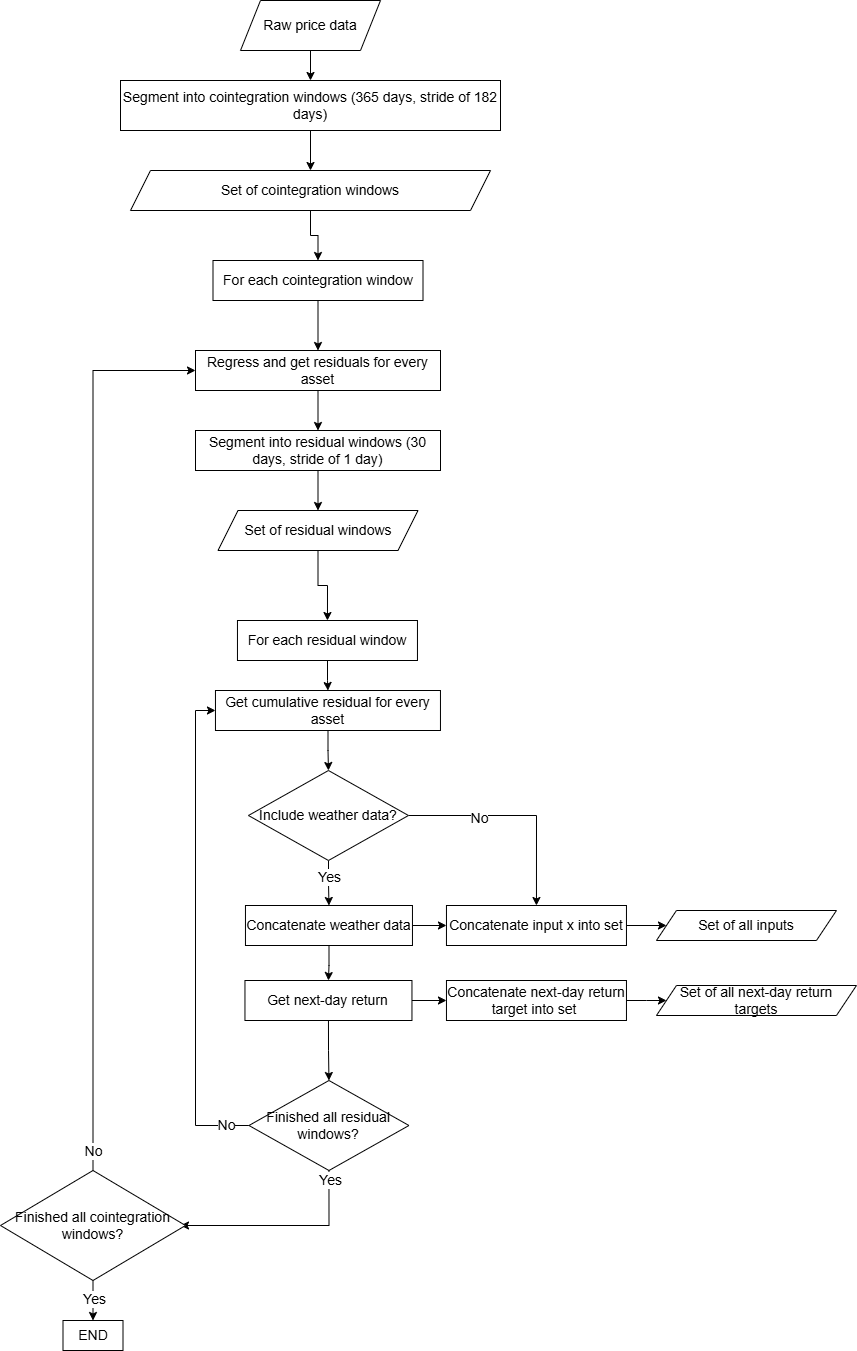
\includegraphics[width=0.8\textwidth]{assets/input_preparation_pipeline.drawio.png}
    \caption{Input Preparation Pipeline for Deep Learning Model}
    \label{fig:input_preparation_pipeline}
\end{figure}

% % Input figure of input preparation pipeline
% \begin{figure}[H]
%     \centering
%     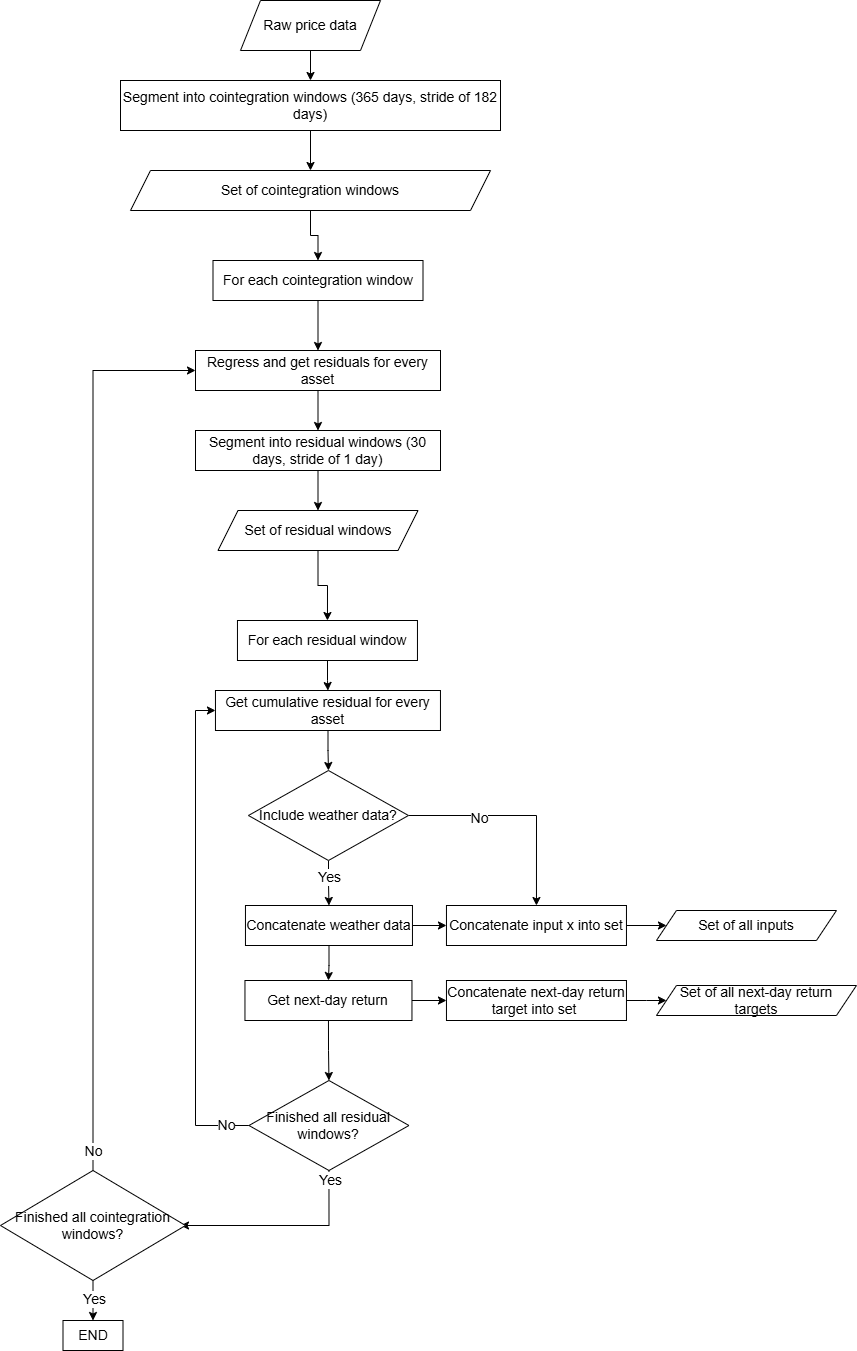
\includegraphics[width=0.8\textwidth]{assets/input_preparation_pipeline.drawio.png}
%     \caption{Input Preparation Pipeline for Deep Learning Model}
%     \label{fig:input_preparation_pipeline}
% \end{figure}

%Input pdf figure of data preparation pipeline
\begin{figure}[t]
    \centering
    \includegraphics[width=0.75\textwidth]{assets/input_preparation_pipeline_example1.pdf}
    \caption{Data Preparation Pipeline for Deep Learning Model (1 of 2, continued on next page)}
    \label{fig:data_preparation_pipeline1}
\end{figure}

\begin{figure}[t]
    \centering
    \includegraphics[width=0.6\textwidth]{assets/input_preparation_pipeline_example2.pdf}
    \caption{Data Preparation Pipeline for Deep Learning Model (2 of 2)}
    \label{fig:data_preparation_pipeline2}
\end{figure}


\begin{figure}
    \centering
    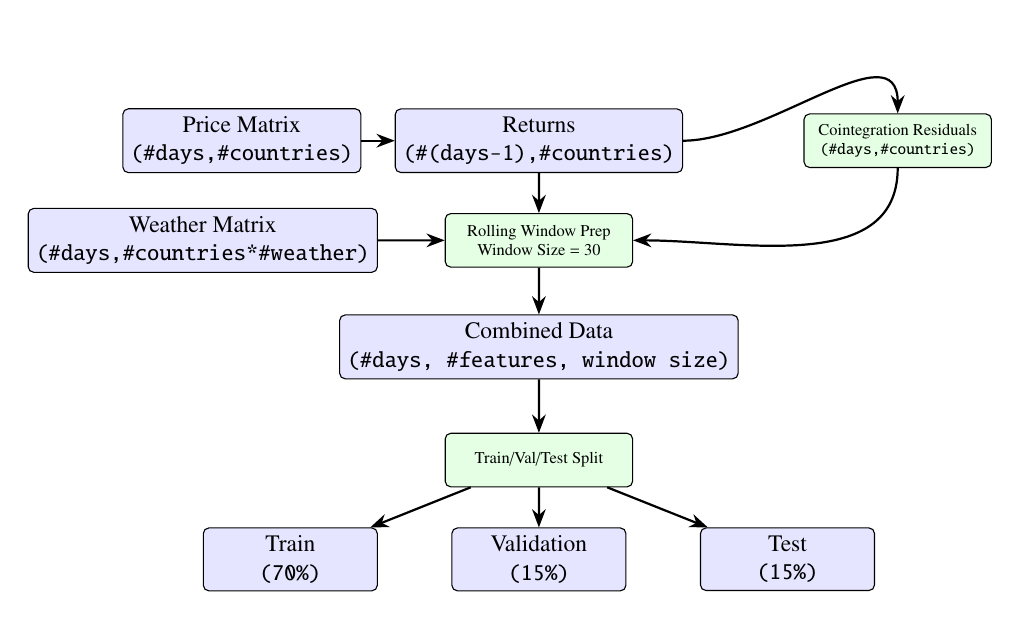
\begin{tikzpicture}[node distance=0.6cm and 0.5cm, scale=0.85, transform shape]
        % Top-level inputs
        \node[data] (price) {Price Matrix\\\texttt{(\#days,\#countries)}};
    
        
        
        \node[data, right=of price] (returns) {Returns\\\texttt{(\#(days-1),\#countries)}};
    
        \node[process, right=1.8cm of returns] (residuals) {Cointegration Residuals\\\texttt{(\#days,\#countries)}};
    
        % Preparation step
        \node[process, below=0.6cm of returns] (prep) {Rolling Window Prep\\Window Size = 30};

        \node[data, left=1cm of prep] (weather) {Weather Matrix\\\texttt{(\#days,\#countries*\#weather)}};
        
        % Combined final data
        \node[data, below=0.7cm of prep] (combined) {Combined Data\\\texttt{(\#days, \#features, window size)}};
    
        % Train/val/test split
        \node[process, below=0.8cm of combined] (split) {Train/Val/Test Split};
        \node[data, below left=0.6cm and 1.0cm of split] (train) {Train\\\texttt{(70\%)}};
        \node[data, below=0.6cm of split] (val) {Validation\\\texttt{(15\%)}};
        \node[data, below right=0.6cm and 1.0cm of split] (test) {Test\\\texttt{(15\%)}};
    I 
        % Arrows
        \draw[arrow] (price) -- (returns);
        \draw[arrow] (weather) -- (prep);
        \draw[arrow] (returns) -- (prep);
        \draw[arrow] (returns.east) to[out=0, in=90] (residuals.north);
        \draw[arrow] (residuals.south) to[out=-90, in=0] (prep.east);
    
        \draw[arrow] (prep) -- (combined);
        %\draw[arrow] (inputs.north) to[out=90, in=180] ([xshift=-0.8cm]combined.north);
        %\draw[arrow] (nextday.north) to[out=90, in=0] ([xshift=0.8cm]combined.north);
    
        \draw[arrow] (combined) -- (split);
        \draw[arrow] (split) -- (train);
        \draw[arrow] (split) -- (val);
        \draw[arrow] (split) -- (test);
    \end{tikzpicture}                     
    \caption{Data Processing Pipeline}
    \label{data_processing_pipeline}
\end{figure}

\begin{figure}
    \centering
    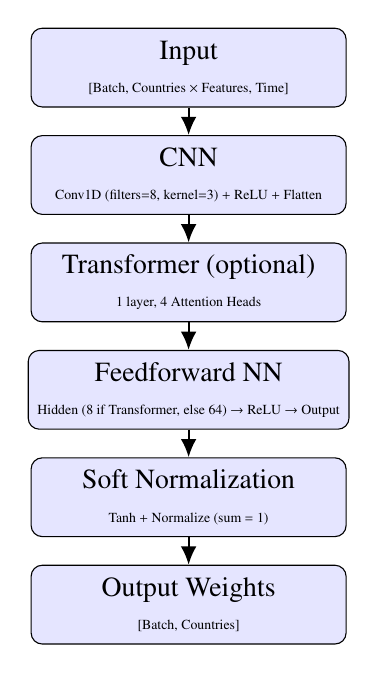
\begin{tikzpicture}[
      node distance=0.35cm,
      box/.style={draw, rounded corners, align=center, minimum height=1cm, minimum width=4cm, fill=blue!10},
      arrow/.style={-{Latex[width=2mm]}, thick}
    ]
    
    \node[box] (input) {Input\\{\tiny [Batch, Countries × Features, Time]}};
    \node[box, below=of input] (cnn) {CNN\\{\tiny Conv1D (filters=8, kernel=3) + ReLU + Flatten}};
    \node[box, below=of cnn] (transformer) {Transformer (optional) \\{\tiny 1 layer, 4 Attention Heads}};
    \node[box, below=of transformer] (ffn) {Feedforward NN\\{\tiny Hidden (8 if Transformer, else 64) → ReLU → Output}};
    \node[box, below=of ffn] (norm) {Soft Normalization\\{\tiny Tanh + Normalize (sum = 1)}};
    \node[box, below=of norm] (output) {Output Weights\\{\tiny [Batch, Countries]}};
    
    \draw[arrow] (input) -- (cnn);
    \draw[arrow] (cnn) -- (transformer);
    \draw[arrow] (transformer) -- (ffn);
    \draw[arrow] (ffn) -- (norm);
    \draw[arrow] (norm) -- (output);
    
    \end{tikzpicture}

    \caption{Model Architecture Overview}
    \label{model_architecture}
\end{figure}

\begin{figure}
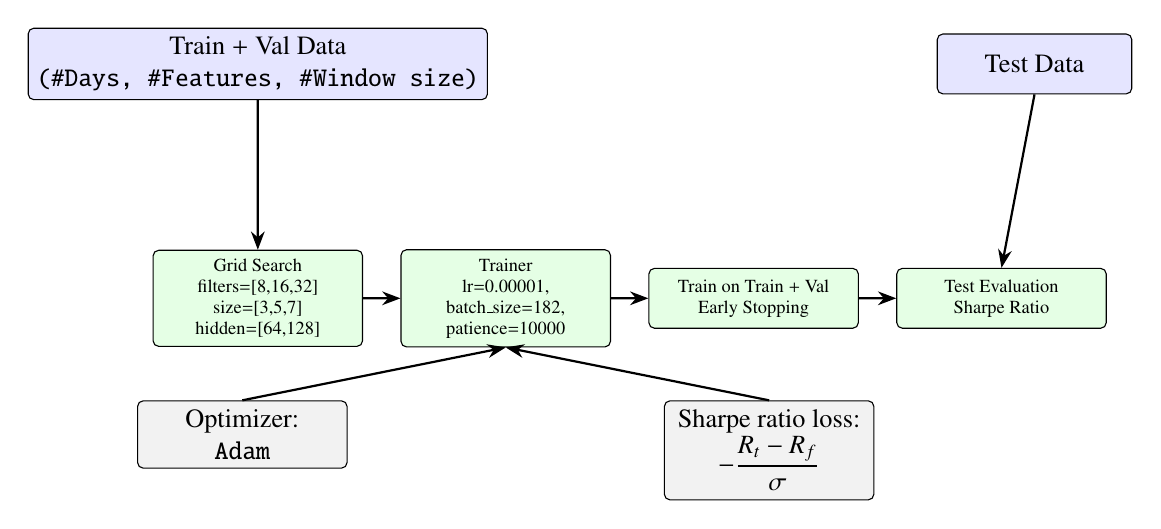
\begin{tikzpicture}[node distance=1cm and 0.5cm, scale=0.95, transform shape]

    % Top Row: Input Data
    \node[data] (train_data) {Train + Val Data\\\texttt{(\#Days, \#Features, \#Window size)}};
    \node[data, right=6 cm of train_data] (test_data) {Test Data};

    % Middle Row: Training Stages
    \node[process, below=2cm of train_data] (grid_search) {Grid Search\\ filters=[8,16,32]\\size=[3,5,7]\\hidden=[64,128]};
    \node[process, right=of grid_search] (trainer) {Trainer\\ lr=0.00001, \\batch\_size=182, \\ patience=10000};
    \node[process, right=of trainer] (train_val) {Train on Train + Val\\Early Stopping};
    \node[process, right=of train_val] (test) {Test Evaluation\\Sharpe Ratio};

    % % Custom Loss Function (below Trainer)
    \node[loss, below right= 1 cm of trainer] (loss_fn) {Sharpe ratio loss: \\\texttt{$-\dfrac{R_t - R_f}{\sigma}$}};

    % % Custom Loss Function (below Trainer)
    \node[loss, below left= 1 cm of trainer] (optimizer) {Optimizer: \\\texttt{Adam}};

    % Arrows: Data Inputs
    \draw[arrow] (train_data) -- (grid_search);
    \draw[arrow] (test_data.south) -- (test.north);

    % Arrows: Process Flow
    \draw[arrow] (grid_search) -- (trainer);
    \draw[arrow] (trainer) -- (train_val);
    \draw[arrow] (train_val) -- (test);

    % Arrow: Trainer uses Custom Loss
    \draw[arrow] (loss_fn.north) -- (trainer.south);
    \draw[arrow] (optimizer.north) -- (trainer.south);
    
    \end{tikzpicture}
    \caption{Training and Evaluation}
    \label{training_and_evaluation}
\end{figure}





\end{document}
